%Master File:lectures.tex

\lesson{Convexity}
\vspace{-1cm}
\begin{center}
  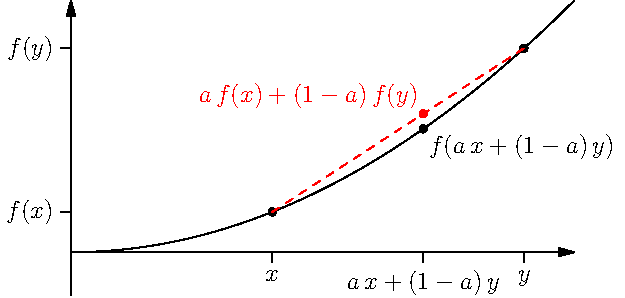
\includegraphics[width=0.5\linewidth]{convex-4}
\end{center}
\keywords{Convex sets, convex functions, Jensen's inequality}
%%%%%%%%%%%%%%%%%%%%%%% Next Slide %%%%%%%%%%%%%%%%%%%%%%%
\renewcommand{\Outline}{%
\begin{slide}
\section[1]{Outline}

\begin{minipage}{12cm}\raggedright
  \begin{enumerate}\squeeze
    \outlineitem{Convex sets}{convexsets}
    \outlineitem{Convex functions}{convexregions}
    \outlineitem{Jensen's inequality}{jensen}
  \end{enumerate}
\end{minipage}\hfill
\begin{minipage}{10cm}
  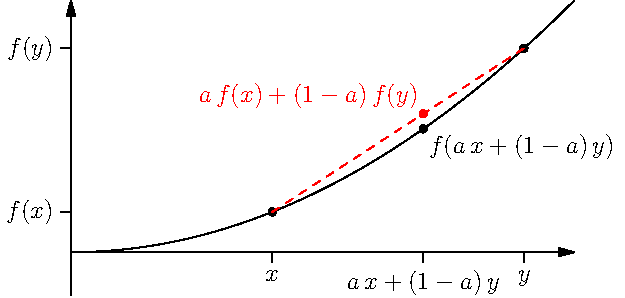
\includegraphics[width=10cm]{convex-4}
\end{minipage}
\end{slide}
\addtocounter{outlineitem}{1}
}

\setcounter{outlineitem}{1}

%%%%%%%%%%%%%%%%%%%%%%% Next Slide %%%%%%%%%%%%%%%%%%%%%%%
\Outline % Convex Sets
%%%%%%%%%%%%%%%%%%%%%%% Next Slide %%%%%%%%%%%%%%%%%%%%%%%

\begin{slide}
\section{Convex Regions}

\begin{rightImage}[0.15]{convexRegion}
\begin{PauseHighLight}
  \begin{itemize}
  \item Convex regions are familiar\hfill\raisebox{-2cm}{
    \includegraphics[width=0.3\linewidth]{convex-region}}\hfill\pause
  \item For any two points $\bm{x}$ and $\bm{y}$ in a region
    $\mathcal{R}$ then for any $a\in[0,1]$ if
    \begin{align*}
      \bm{z} = a\,\bm{x} + (1-a)\,\bm{y} \in \mathcal{R}
    \end{align*}
  \item then $\mathcal{R}$ is a convex region\pause
  \end{itemize}
\end{PauseHighLight}
\end{rightImage}

\end{slide}

%%%%%%%%%%%%%%%%%%%%%%% Next Slide %%%%%%%%%%%%%%%%%%%%%%%

\begin{slide}
\section{Convex Sets}

\begin{PauseHighLight}
  \begin{itemize}
  \item For any set, $\mathcal{S}$, where addition and scalar
    multiplication is defined (e.g. a vector space) then:
    \begin{quotation}
      \noindent If for any two elements $\bm{x},\bm{y} \in \mathcal{S}$ and any
      $a\in[0,1]$
      \begin{align*}
        \bm{z} = a\,\bm{x} + (1-a)\,\bm{y} \in \mathcal{S}
      \end{align*}
      then $\mathcal{S}$ is said to be a convex set\pause
    \end{quotation}
  \end{itemize}
\end{PauseHighLight}

\end{slide}

%%%%%%%%%%%%%%%%%%%%%%% Next Slide %%%%%%%%%%%%%%%%%%%%%%%

\begin{slide}
\section[-2]{Positive Semi-Definite Matrices}

\begin{PauseHighLight}
  \begin{itemize}
  \item Recall that a matrix $\mat{M}$ is positive semi-definite if for any
    vector $\bm{v}$
    \begin{align*}
      \bm{v}^\tr \mat{M}\,\bm{v} \geq 0\pause
    \end{align*}
    (i.e.{} any quadratic form of the matrix is non-negative)\pauseb
  \item (We showed this also implies that all the eigenvalues are
    non-negative)\pause
  \item We denote the fact that $\mat{M}$ is positive semi-definite by
    $\mat{M}\succeq0$, and $\mat{M} \succ 0$ if it is positive definite\pause
  \item The set of positive semi-definite (PSD) matrices (or kernels) form a
    convex set\pause
  \end{itemize}
\end{PauseHighLight}


\end{slide}

%%%%%%%%%%%%%%%%%%%%%%% Next Slide %%%%%%%%%%%%%%%%%%%%%%%

\begin{slide}
\section[-2]{Proof}

\begin{PauseHighLight}
  \begin{itemize}
  \item Consider any two arbitrarily chosen PSD matrices $\mat{M}_1$
    and $\mat{M}_2$ and any $a\in[0,1]$ then let
    \begin{align*}
      \mat{M}_3 = a\,\mat{M}_1 + (1-a)\,\mat{M}_2\pause
    \end{align*}
  \item Then for any vector $\bm{v}$
    \begin{align*}
      \bm{v}^\tr \mat{M}_3 \bm{v}
      &= \bm{v}^\tr \left(  a\,\mat{M}_1 + (1-a)\,\mat{M}_2\right)
        \bm{v} \pause\\
      &=
        a\, \bm{v}^\tr \mat{M}_1 \bm{v} + (1-a)  \bm{v}^\tr \mat{M}_2
        \bm{v}\pause\\
      &= a\,m_1 + (1-a)\,m_2
    \end{align*}
    where $m_1 = \bm{v}^\tr \mat{M}_1 \bm{v}$ and $m_2 = \bm{v}^\tr
    \mat{M}_2 \bm{v}$\pause
  \item But $m_1,m_2\geq 0$ since $\mat{M}_1, \mat{M}_2 \succeq 0$.\pause{}  Thus $a\,m_1 + (1-a)\,m_2\geq 0$ and so
    $\mat{M}_3\succeq 0 \quad\square$\pause
  \end{itemize}
\end{PauseHighLight}

\end{slide}



%%%%%%%%%%%%%%%%%%%%%%% Next Slide %%%%%%%%%%%%%%%%%%%%%%%
\Outline % Convex Sets
%%%%%%%%%%%%%%%%%%%%%%% Next Slide %%%%%%%%%%%%%%%%%%%%%%%

\begin{slide}
  \section[-2]{Convex Functions}

  \pb
  \begin{itemize}
  \item Any function $f(x)$ is said to be a \emph{convex function} if
    for any two points $x$ and $y$ and any $a\in[0,1]$
    \begin{align*}
      f(a \,x + (1-a)\, y) \leq a f(x) + (1-a) f(y)\pause
    \end{align*}
    \begin{center}
      \multipdf[width=0.8\linewidth]{convex}\pause
    \end{center}
  \end{itemize}
\end{slide}

%%%%%%%%%%%%%%%%%%%%%%% Next Slide %%%%%%%%%%%%%%%%%%%%%%%

\begin{slide}
\section[-2]{Epigraph}

\begin{PauseHighLight}
  \begin{itemize}
  \item The \emph{epigraph} of a function is the area that lies above
    the function\pause
  \item The epigraph of a convex function is a convex region
    \begin{center}
      \multipdf[width=0.8\linewidth]{epigraph}\pauseb
    \end{center}
  \end{itemize}
\end{PauseHighLight}

\end{slide}

%%%%%%%%%%%%%%%%%%%%%%% Next Slide %%%%%%%%%%%%%%%%%%%%%%%

\begin{slide}
\section[-2]{Convex-Down or Concave Functions}

\begin{PauseHighLight}
  \begin{itemize}
  \item Any function, $f(x)$, that satisfies the inverse inequality
    \begin{align*}
      f(a \,x + (1-a)\, y) \geq a f(x) + (1-a) f(y)\pause
    \end{align*}
    for any points $x$ and $y$ and any $a\in[0,1]$ is said to be a
    \emph{convex-down} or \emph{concave} function\pause
  \item Everything true for a convex(-up) function carries over to a
    convex-down function with a small modification\pause
  \item If $f(x)$ is a convex-up function then $g(x)=-f(x)$ is a
    convex-down function\pause
  \item The area that lies below a convex-down function is a convex
    region\pause
  \end{itemize}
\end{PauseHighLight}

\end{slide}

%%%%%%%%%%%%%%%%%%%%%%% Next Slide %%%%%%%%%%%%%%%%%%%%%%%

\begin{slide}
\section[-2]{Examples}

\pb\pause
\pauselevel{=1}
\begin{center}
  \multipdf[width=\linewidth]{examplesConvexity}\pause
\end{center}
\end{slide}

%%%%%%%%%%%%%%%%%%%%%%% Next Slide %%%%%%%%%%%%%%%%%%%%%%%

\begin{slide}
\section[-2]{Linear Functions}

\begin{PauseHighLight}
  \begin{itemize}
  \item Linear functions are given by
    \begin{align*}
      f(x) = m\,x + c\pause
    \end{align*}
  \item They satisfy the \emph{equality}
    \begin{align*}
      f(a \,x + (1-a)\, y) = a f(x) + (1-a) f(y)\pause
    \end{align*}
  \item As such they are both convex(-up) and convex-down
    function\pause    
  \item $|x|$ is a convex-up function \raisebox{-1cm}{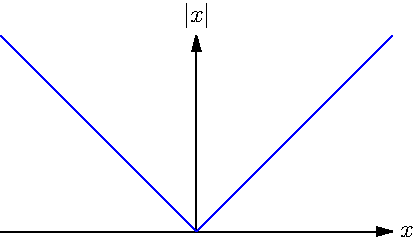
\includegraphics[width=0.3\linewidth]{modx}}\pause
  \end{itemize}
\end{PauseHighLight}

\end{slide}

%%%%%%%%%%%%%%%%%%%%%%% Next Slide %%%%%%%%%%%%%%%%%%%%%%%

\begin{slide}
\section{Strictly Convex Function}

\begin{PauseHighLight}
  \begin{itemize}
  \item Functions that satisfy the strict inequality (for $0<a<1$ and
    $x\neq y$)
    \begin{align*}
      f(a \,x + (1-a)\, y) < a f(x) + (1-a) f(y)
    \end{align*}
    are said to be \emph{strictly convex functions}\pause
  \item A strictly convex-down function satisfies the reverse strict
    inequality\pause
  \item Strictly convex-(up or down) functions don't contain any
    linear regions\pause
  \end{itemize}
\end{PauseHighLight}

\end{slide}


%%%%%%%%%%%%%%%%%%%%%%% Next Slide %%%%%%%%%%%%%%%%%%%%%%%

\begin{slide}
\section{Convexity in High Dimensions}

\begin{PauseHighLight}
  \begin{itemize}
  \item If $f:\mathbb{R}^n \to \mathbb{R}$ (i.e. $f(\bm{x})$ maps
    high dimensional point $\bm{x}\in \mathbb{R}^n$ to a real value)
    satisfies
    \begin{align*}
      f(a \,\bm{x} + (1-a)\, \bm{y}) \leq  a \, f(\bm{x}) + (1-a) \, f(\bm{y})
    \end{align*}
    for any $\bm{x}, \bm{y}\in \mathbb{R}^n$ and any $a\in[0,1]$
    then $f(\bm{x})$ is a convex function\pause
  \item $\|\bm{x}\|_2^2 = \sum\limits_i x_i^2$ is a (strictly) convex function\pause
  \item $\|\bm{x}\|_1 = \sum\limits_i |x_i|$ is a convex function\pause
  \end{itemize}
\end{PauseHighLight}

\end{slide}


%%%%%%%%%%%%%%%%%%%%%%% Next Slide %%%%%%%%%%%%%%%%%%%%%%%

\begin{slide}
\section[-2]{Properties of Convex Functions}

\pb
\begin{itemize}
\item Convex functions lie on or above any tangent line
  \begin{align*}
    f(x) \geq f(x^*) + (x-x^*) f'(x^*)\pause
  \end{align*}
  \begin{center}
    \multipdf[width=0.9\linewidth]{aboveGrad}\pauseb
  \end{center}
\end{itemize}

\end{slide}

%%%%%%%%%%%%%%%%%%%%%%% Next Slide %%%%%%%%%%%%%%%%%%%%%%%

\begin{slide}
\section[-2]{Second Derivatives}

\begin{PauseHighLight}
  \begin{itemize}
  \item As $f(x)$ lies on or above its tangent line then for any $\epsilon>0$
    \begin{align*}
      f'(x+\epsilon)\geq f'(x)\pause
    \end{align*}
    therefore $f''(x) = \lim_{\epsilon\rightarrow0} (f'(x+\epsilon)-
    f'(x))/\epsilon \geq 0$ at all points $x$\pause
  \item In high dimensions a convex function lies above its tangent plane
    \begin{align*}
      f(\bm{x}) \geq f(\bm{x}^*) + (\bm{x}-\bm{x}^*)^\tr \grad f(\bm{x}^*)\pause
    \end{align*}
  \item The matrix of second derivatives (the Hessian) must be
    positive semi-definite at all points $\bm{x}$
    {\small \begin{align*}
      \mat{H} =
      \begin{pmatrix}
        \pd[2]{f(\bm{x})}{x_1^2} & \pd[2]{f(\bm{x})}{x_1\, \partial
          x_2} & \ldots \\
        \pd[2]{f(\bm{x})}{x_2 \, \partial x_1} &
        \pd[2]{f(\bm{x})}{x_2^2} & \ldots\\
        \vdots & \vdots & \ddots
      \end{pmatrix} \succeq 0\pause
    \end{align*} }
  \end{itemize}
\end{PauseHighLight}

\end{slide}

%%%%%%%%%%%%%%%%%%%%%%% Next Slide %%%%%%%%%%%%%%%%%%%%%%%

\begin{slide}
\section[-2]{Proving Convexity}

\begin{PauseHighLight}\squeeze
  \begin{itemize}
  \item $f(x)=x^2$ is strictly convex as $f''(x)=2>0$\pause
  \item $f(x)=\e{c\,x}$ is strictly convex as $f''(x) =
    c^2\,\e{c\,x}>0$\pause
  \item $f(x) = \log(x)$ is strictly convex-down
    as $f''(x)=-\frac{1}{x^2}<0$\pause
  \item $f(x,y) = \frac{x^2}{y}$ is convex for $y>0$ as
    \begin{align*}
      \mat{H} =
      \begin{pmatrix}
        \frac{\partial^2 f(x,y)}{\partial x^2}
        &
        \frac{\partial^2 f(x,y)}{\partial x \partial y}\\
        \frac{\partial^2 f(x,y)}{\partial y \partial x}
        &
        \frac{\partial^2 f(x,y)}{\partial y^2}
      \end{pmatrix}
      =
          \begin{pmatrix}
            \frac{2}{y}
            & -\frac{2\,x}{y^2} \\
            -\frac{2\,x}{y^2}
            & \frac{2\,x^2}{y^3}
          \end{pmatrix}
              = \frac{2}{y^3}
              \begin{pmatrix}
                y^2 & -x\,y \\
                -x\,y & x^2
              \end{pmatrix}\pause
    \end{align*}
  \item Now $T = \mathrm{tr}\, \mat{H} = \frac{2}{y^3}(x^2+y^2)$, $D =
    \det(\mat{H})=0$\pause
  \item $\lambda_{1,2} =T/2 \pm \sqrt{T^2/4-D} = \{0, T\} =
    \{0,\frac{2(x^2+y^2)}{y^3}\} \geq 0 \Rightarrow \mat{H}\succeq 0$\pause
  \end{itemize}
\end{PauseHighLight}

\end{slide}

%%%%%%%%%%%%%%%%%%%%%%% Next Slide %%%%%%%%%%%%%%%%%%%%%%%

\begin{slide}
\section[-2]{Sums of Convex Functions}

\begin{PauseHighLight}
  \begin{itemize}
  \item For any set of convex functions $f_1(x)$, $f_2(x)$, $\ldots$
    and any set of non-negative scalars $a_1$, $a_2$, $\ldots$ then
    \begin{align*}
      g(x) = \sum_i a_i\,f_i(x)
    \end{align*}
    is convex\pause
  \item Proof
    \begin{align*}
      g''(x) = \sum_i a_i \, f_i''(x)
    \end{align*}
    but $f_i''(x)\geq 0$ so $g''(x)$ is a sum on non-negative
    terms\pause
  \item This generalises to higher dimensions as the sum of PSD
    matrices times positive factors is a PSD matix\pause
  \end{itemize}
\end{PauseHighLight}
  

\end{slide}


%%%%%%%%%%%%%%%%%%%%%%% Next Slide %%%%%%%%%%%%%%%%%%%%%%%

\begin{slide}
\section[-2]{Convex Functions Defined on Convex Sets}

\pb
\begin{itemize}
\item All the properties we have discussed hold for functions
  defined on a convex set\pauseh
\item $\sin(x)$ is not generally neither convex up or down\pauseh
\item $\sin(x)$ for $x\in[0, \pi]$ is convex-down\pauseh{} (its second
  derivative $-\sin(x)$ is less than or equal to 0 in this
  range)\pause
  \begin{center}
    \multipdf[width=0.75\linewidth]{sinConvex}\pause
  \end{center}\pauselevel{=7}
\item For a convex function defined on a non-convex set,
  $\mathcal{S}$, there exists points $\bm{x},\bm{y} \in \mathcal{S}$
  such that for some $a\in[0,1]$ there will be points
  $\bm{z}=a\,\bm{x}+(1-a)\bm{y}\not\in\mathcal{S}$\pauseh{} (the
  function isn't defined on such points)\pause
\end{itemize}
  

\end{slide}

%%%%%%%%%%%%%%%%%%%%%%% Next Slide %%%%%%%%%%%%%%%%%%%%%%%

\begin{slide}
\section{Constraints}

\begin{PauseHighLight}
  \begin{itemize}
  \item Often we impose constraints on the set of points, e.g.
    \begin{align*}
      x_i &> 0  & \bm{a}^\tr \bm{x} &= b & \bm{x}^\tr \mat{M}
                                           \, \bm{x} &\leq 1\pause
    \end{align*}
  \item Linear constraints (e.g. $x_i > 0$ or $\bm{a}^\tr \bm{x} =
    b$ or $\bm{a}^\tr \bm{x} \leq b$) always define a
    convex region\pause
  \item Multiple linear constraints always define a convex region\pause
  \item Non-linear constraints may or may not define a convex
    region\pause{} ($\{\bm{x} \in \mathbb{R}^n|\bm{x}^\tr \mat{M}\, \bm{x}
    \leq 1, \mat{M}\succeq 0\}$ does while
     $\{\bm{x} \in \mathbb{R}^n|\bm{x}^\tr \mat{M}\, \bm{x}
    \geq 1, \mat{M}\succeq 0\}$ doesn't)\pauseb
  \end{itemize}
\end{PauseHighLight}
  

\end{slide}



%%%%%%%%%%%%%%%%%%%%%%% Next Slide %%%%%%%%%%%%%%%%%%%%%%%

\begin{slide}
\section[-1]{Unique Minimum}

\begin{PauseHighLight}
  \begin{itemize}
  \item Strictly convex function have a unique minimum\pause
  \item The existence of a local minimum would break convexity\pause

    \begin{rightImage}{doubleDip}
      \begin{itemize}
      \item The line connecting a local minimum to a global minimum
        would be strictly decreasing\pause
      \item Thus there are points next to the local minimum with lower
        values\pause
      \item This is a contradiction\pause
      \end{itemize}
    \end{rightImage}

  \item This remains true if we consider convex functions that are
    constrained to live in a convex set\pause
  \end{itemize}
\end{PauseHighLight}

\end{slide}

%%%%%%%%%%%%%%%%%%%%%%% Next Slide %%%%%%%%%%%%%%%%%%%%%%%

\begin{slide}
\section{Convex Set of Minima}

\begin{PauseHighLight}
  \begin{itemize}
  \item If $f(\bm{x})$ is \emph{convex} but not \emph{strictly convex}
    then there might exist a convex set
    $\mathcal{M}\subset\mathcal{X}$ of minima such that for all
    $\bm{x}, \bm{y} \in \mathcal{M}$ and any $\bm{z} \in \mathcal{X}$
    we have $f(\bm{x})=f(\bm{y}) \leq f(\bm{z})$\pause
  \item This set of minima is convex, that is, if $\bm{x}, \bm{y}
    \in \mathcal{M}$ then for any $a\in[0,1]$ the point
    $\bm{z}=a\,\bm{x} + (1-a)\, \bm{y}\in \mathcal{M}$\pause
  \item The sum of a convex function, $f(x)$, and a strictly convex function
    $g(x)$ will always be strictly convex since
    \begin{align*}
      f''(x) + g''(x) >0 
    \end{align*}
    as $f''(x)\geq 0$ and $g''(x)>0$\pause
  \end{itemize}
\end{PauseHighLight}

\end{slide}


%%%%%%%%%%%%%%%%%%%%%%% Next Slide %%%%%%%%%%%%%%%%%%%%%%%

\begin{slide}
\section{Linear Regression}

\begin{PauseHighLight}
  \begin{itemize}
  \item For linear regression the loss function
    \begin{align*}
      L(\bm{w}) = \| \mat{X}\, \bm{w} - \bm{y} \|^2 = \bm{w}^\tr
      \mat{X}^\tr\mat{X} \bm{w} - 2 \bm{w}^\tr \mat{X}^\tr\, \bm{y} +
      \bm{y}^\tr \bm{y}
    \end{align*}
    is convex\pause
  \item Since the Hessian $\mat{H} = 2\,\bm{X}^\tr \bm{X} \succeq 0$
    (positive semi-definite)\pause\\
    (For any vector $\bm{v}$ then $\bm{v}^\tr \mat{H} \bm{v} =
    2\,\bm{v}^\tr\mat{X}^\tr \mat{X}\bm{v} = 2\,\| \mat{X}\bm{v} \|^2 \geq 0$)\pauseb
  \item If $\mat{H}\succ 0$ there will be a unique minima\pause, while
    if $\mat{H}$ has some zero eigenvalues there will be a family of
    solutions\pauseb
  \end{itemize}
\end{PauseHighLight}

\end{slide}

%%%%%%%%%%%%%%%%%%%%%%% Next Slide %%%%%%%%%%%%%%%%%%%%%%%

\begin{slide}
  \section[-2]{Regularised Linear Regression}

\begin{PauseHighLight}
  \begin{itemize}
  \item In ridge regression we minimise a loss
    \begin{align*}
      \hspace{-1cm} L(\bm{w}) = \| \mat{X}\, \bm{w} - \bm{y} \|^2 + \eta\,\|\bm{w}\|^2 = \bm{w}^\tr
      \left( \mat{X}^\tr\mat{X} + \eta \mat{I}\right) \bm{w} - 2 \bm{w}^\tr \mat{X}^\tr\, \bm{y} +
      \bm{y}^\tr \bm{y}\pause
    \end{align*}
  \item Because $\|\bm{w}\|^2$ is strictly convex the loss function is
    strictly convex and so will have a unique solution\pause
  \item Using an $L_1$ regulariser (Lasso)
    \begin{align*}
           L(\bm{w}) = \| \mat{X}\, \bm{w} - \bm{y} \|^2 + \eta\,\|\bm{w}\|_1
    \end{align*}
    again $\|\bm{w}\|_1$ is convex and so $L(\bm{w})$ will be convex\pause
  \item Using an $L_1$ and an $L_2$ regulariser (elastic net) also
    gives a unique solution\pause    
  \end{itemize}
\end{PauseHighLight}

\end{slide}


%%%%%%%%%%%%%%%%%%%%%%% Next Slide %%%%%%%%%%%%%%%%%%%%%%%
\Outline % Jensen's Inequality
%%%%%%%%%%%%%%%%%%%%%%% Next Slide %%%%%%%%%%%%%%%%%%%%%%%

\begin{slide}
\section{Jensen's Inequality}

\begin{PauseHighLight}
  \begin{itemize}
  \item In proving many properties of learning machines inequalities
    are really useful\pause
  \item One of the most useful inequalities involve expectations of
    convex functions, this is known as \emph{Jensen's
      Inequality}\pause
  \item If $f(\bm{x})$ is a convex(-up) function then
    \begin{align*}
      \av{f(\bm{X})} \geq f(\av{\bm{X}})\pause
    \end{align*}
  \item If $f(\bm{x})$ is a convex(-down) function then
    \begin{align*}
      \av{f(\bm{X})} \leq f(\av{\bm{X}})\pauseb
    \end{align*}
  \end{itemize}
\end{PauseHighLight}

\end{slide}

%%%%%%%%%%%%%%%%%%%%%%% Next Slide %%%%%%%%%%%%%%%%%%%%%%%

\begin{slide}
\section{Proof}

\begin{PauseHighLight}
  \begin{itemize}
  \item We said before that a convex function must lie on or above its
    tangent plane at any point $\bm{x}^*$
    \begin{align*}
      f(\bm{x}) \geq f(\bm{x}^*) + (\bm{x}-\bm{x}^*)^\tr \grad f(\bm{x}^*)\pause
    \end{align*}
  \item Taking $\bm{x}^*=\av{\bm{X}}$
    \begin{align*}
      f(\bm{X}) \geq f(\av{\bm{X}}) + (\bm{X}-\av{\bm{X}})^\tr \grad f(\av{\bm{X}})\pause
    \end{align*}
  \item Taking expectations of both sides
    \begin{align*}
      \av{f(\bm{X})}
      &\geq f(\av{\bm{X}}) +
      (\av{\bm{X}}-\av{\bm{X}})^\tr \grad f(\av{\bm{X}})\pause\\
      &= f(\av{\bm{X}}) \hspace{10cm} \square\pauseb
    \end{align*}
  \end{itemize}
\end{PauseHighLight}

\end{slide}

%%%%%%%%%%%%%%%%%%%%%%% Next Slide %%%%%%%%%%%%%%%%%%%%%%%

\begin{slide}
\section{Simple Proofs with Jensen's Inequality}

\begin{PauseHighLight}
  \begin{itemize}
  \item Since $f(x) = x^2$ is convex by Jensen's inequality
    \begin{align*}
      \av{X^2} \geq  (\av{X})^2\pause \quad \text{or} \quad
      \av{X^2}-\av{X}^2 \geq 0
    \end{align*}
    (i.e. variance are non-negative)\pause
  \item The KL-divergence $\mathrm{KL}(f \| g)$ between two
    categorical probability distributions $(f_1,f_2,\ldots)$ and
    $(g_1,g_2,\ldots)$ is define as
    \begin{align*}
      \mathrm{KL}(f \| g) = - \sum_i f_i \, \logg{\frac{g_i}{f_i}}
    \end{align*}
    (note $f_i,g_i\geq 0$ and $\sum\limits_i f_i = \sum\limits_i g_i
    =1 $)\pause
  \end{itemize}
\end{PauseHighLight}

\end{slide}

%%%%%%%%%%%%%%%%%%%%%%% Next Slide %%%%%%%%%%%%%%%%%%%%%%%

\begin{slide}
\section[-2]{Kullback-Leibler Divergence}

\pb\pause\pauselevel{=1}
\begin{center}
  \multipdf[width=0.9\linewidth]{klcat}\pause
\end{center}
\end{slide}


%%%%%%%%%%%%%%%%%%%%%%% Next Slide %%%%%%%%%%%%%%%%%%%%%%%

\begin{slide}
  \section[-1]{Proof of Gibbs' Inequality}

  \begin{PauseHighLight}
  \begin{itemize}
  \item To show that $\mathrm{KL}(f \| g)\geq 0$ (Gibbs' inequality) we
    note that since the logarithm is a convex-down function
    \begin{align*}
      \mathrm{KL}(f \| g)
      &= - \sum_i f_i \, \logg{\frac{g_i}{f_i}} \pause
        = \av[f]{-\logg{\frac{g_i}{f_i}}}\pauseb\\
      &\geq -\logg{\av[f]{\frac{g_i}{f_i}}}\pauseb \\
      &= - \logg{\sum_i f_i \frac{g_i}{f_i}}\pauseb
      = -\logg{\sum_i g_i}\pauseb = -\log(1) \pauseb = 0\pauseb
    \end{align*}
  \item We will meet KL-divergences later on\pauseb
  \end{itemize}
\end{PauseHighLight}


\end{slide}

%%%%%%%%%%%%%%%%%%%%%%% Next Slide %%%%%%%%%%%%%%%%%%%%%%%

\begin{slide}
\section{Lessons}

\begin{PauseHighLight}
  \begin{itemize}
  \item Although we haven't talked much about machine learning,
    convexity is heavily used in many machine learning applications\pause
  \item A lot of ML algorithms involve convex functions\pause{} e.g.{}
    SVMs\pauseb
  \item As such they will have a unique minimum (or a convex set of
    minima)\pause
  \item Convexity is an elegant idea which is relatively easy to
    prove theorems about\pause
  \item One of the most useful tools is Jensen's inequality\pause
  \end{itemize}
\end{PauseHighLight}

\end{slide}


%%% Local Variables:
%%% TeX-master: "lectures"
%%% End:
